\chapter{Lambert $W$ Function} \label{app:lambert-w}
\begin{definition}
    The Lambert $W$ function is a function, $y(x)$, such that the following equation holds
    \[ ye^y = x \]
    where $y$ and $x$ are real. The Lambert $W$ function is denoted as $W_k(x)$, where $k=0,-1$ are its two branches.
\end{definition}
\begin{figure} [htbp]
    \centering
    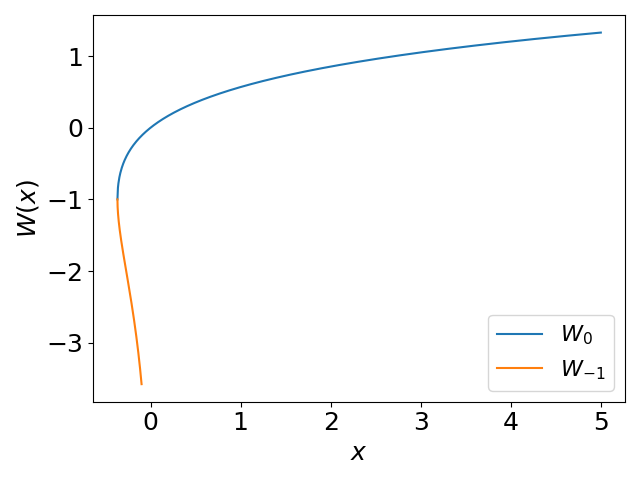
\includegraphics[width=0.7\textwidth]{figures/lambert-w.png}
    \caption{The graph of $y=W(x)$ for real $x<6$ and $y>-4$. The upper branch (blue) with $y\geq-1$ is the graph of the function $W_0(x)$ (principal branch), the lower branch (magenta) with $y\leq -1$ is the graph of the function $W_{-1}(x)$. The minimum value of $x$ is at $(-1/e,-1)$.}
    \label{fig:lambert-w}
\end{figure}